\subsection[Authentification]{Authentification}\label{sec:auth}

\subsubsection[Fortify][laravel.com/docs/12.x/fortify]{Fortify}

Pour cela, nous allons utiliser le package \fortify{} de \laravel{}. 

\textit{``Laravel Fortify is a frontend agnostic authentication backend implementation for Laravel. Fortify registers the routes and controllers needed to implement all of Laravel's authentication features, including login, registration, password reset, email verification, and more''.} (\href{https://laravel.com/docs/12.x/fortify#what-is-fortify}{Doc \laravel})

En gros, c'est une interface utilisateur qui gère l'authentification.

\subsubsection[Installation]{Installation}

C'est plutôt simple, il n'y a rien à faire ! En effet, tout est déjà fourni lors de l'installation de base du projet.

\subsubsection[Configuration]{Configuration}

Avec la version actuelle de \laravel, la configuration se fait très rapidement. Il n'y a, en fait, qu'une seule étape.

\begin{wrapfigure}[5]{r}{0.5\textwidth}
    \vspace{-1cm}
    \colorbox{black}{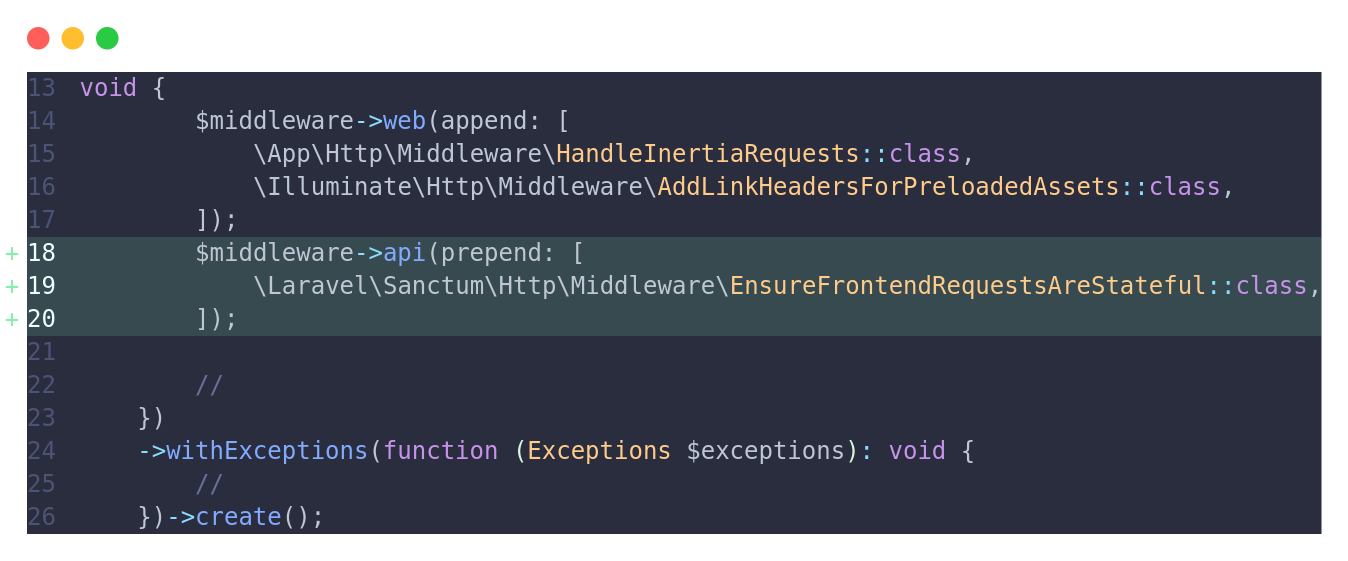
\includegraphics[width=0.5\textwidth]{figures-C1/middleware_app.png}}
\end{wrapfigure}

Ajoutez cette ligne dans \linebreak \verb|boostrap/app.php|. Celle-ci permet à votre navigateur préféré \footnote{Team Firefox, ici} d'utiliser les cookies stockés sur la page pour l'authentification \footnote{Par le biais du X-CSRF-TOKEN}. Plus de détails sur les cookies seront donnés dans la section suivante.

\subsubsection[Cookies]{Cookies}

Les cookies, miam mi... veuillez m'excuser \footnote{Promis, j'arrête.}. Les cookies sont des données sauvegardées sous la forme de texte par votre navigateur. Ils permettent dans notre cas de sauvegarder la session d'un utilisateur mais ont beaucoup d'autres applications comme la mémorisation d'une langue, d'un thème (clair/sombre), d'un panier d'articles, etc. \\

Mais pourquoi diable sommes-nous forcés à accepter/refuser systématiquement les cookies sur tous les sites que nous parcourons ? Les cookies servent aussi à suivre l'activité de l'utilisateur entre les différents sites web, ce qui a bon goût de plaire aux annonceurs qui peuvent connaître nos habitudes et nous envoyer de la publicité ciblée. \\

L'Union Européenne a donc décidé qu'il était obligatoire de laisser le choix à l'utilisateur de consentir ou non à ces cookies absolument pas essentiels au fonctionnement du site web.


\subsubsection[Pages]{Pages} \label{sec:auth_pages}

Nous allons désormais créer les pages de connexion : se connecter, s'inscrire, mot de passe oublié, etc. Mais pas de panique ! Encore une fois, \laravel nous sauve car tout est déjà prémâché pour nous. Dans le dossier \texttt{resources/js/Pages/Auth}, se trouvent 6 pages toutes faites qu'on va exploiter par la suite.

\subsubsubsection[GuestLayout]{GuestLayout}


Mais avant ça, créons un layout commun à toutes les pages comme on a fait pour les pages \texttt{Index}, \texttt{About} et \texttt{Services}. Pour ce faire, créez le fichier \texttt{GuestLayout.jsx} dans \texttt{resources/js/Layouts} et remplissez-le comme la figure \ref{fig:guestlayout}.

\begin{wrapfigure}[2]{r}{0.075\textwidth}
\hspace{0.025\textwidth}
\vspace{-0.75cm}
    \par\medskip
\attachfile[icon=Paperclip,%
            description={Logo N-HiTec},%
            mimetype=image/png]{figures-C1/logo_nhitec.png}

\bigskip
\end{wrapfigure}

Vous remarquerez que le code mentionne un certain fichier \texttt{logo\_nhitec.png}.
Vous pouvez télécharger ce logo attaché au PDF en cliquant sur l'icône suivante \footnote{Ouvrez le panneau "Pièces jointes" de votre lecteur PDF si vous ne voyez pas l'icône ou récupérez la sur le discord \textit{Op\&Ex}.} :

Insérez ensuite cette image dans le dossier \texttt{public}. Ce dernier sert à stocker toutes les données que l'on veut rendre publiques sur notre site web \footnote{Évitez donc, de grâce, d'y insérer quelconque donnée confidentielle.}. Cela tombe bien, c'est exactement ce qu'on veut. Testez vous-même en allant sur \url{http://localhost/logo_nhitec.png}, vous y trouverez le logo de notre chère Junior Entreprise.

\begin{figure}[h]
    \centering
    \colorbox{black}{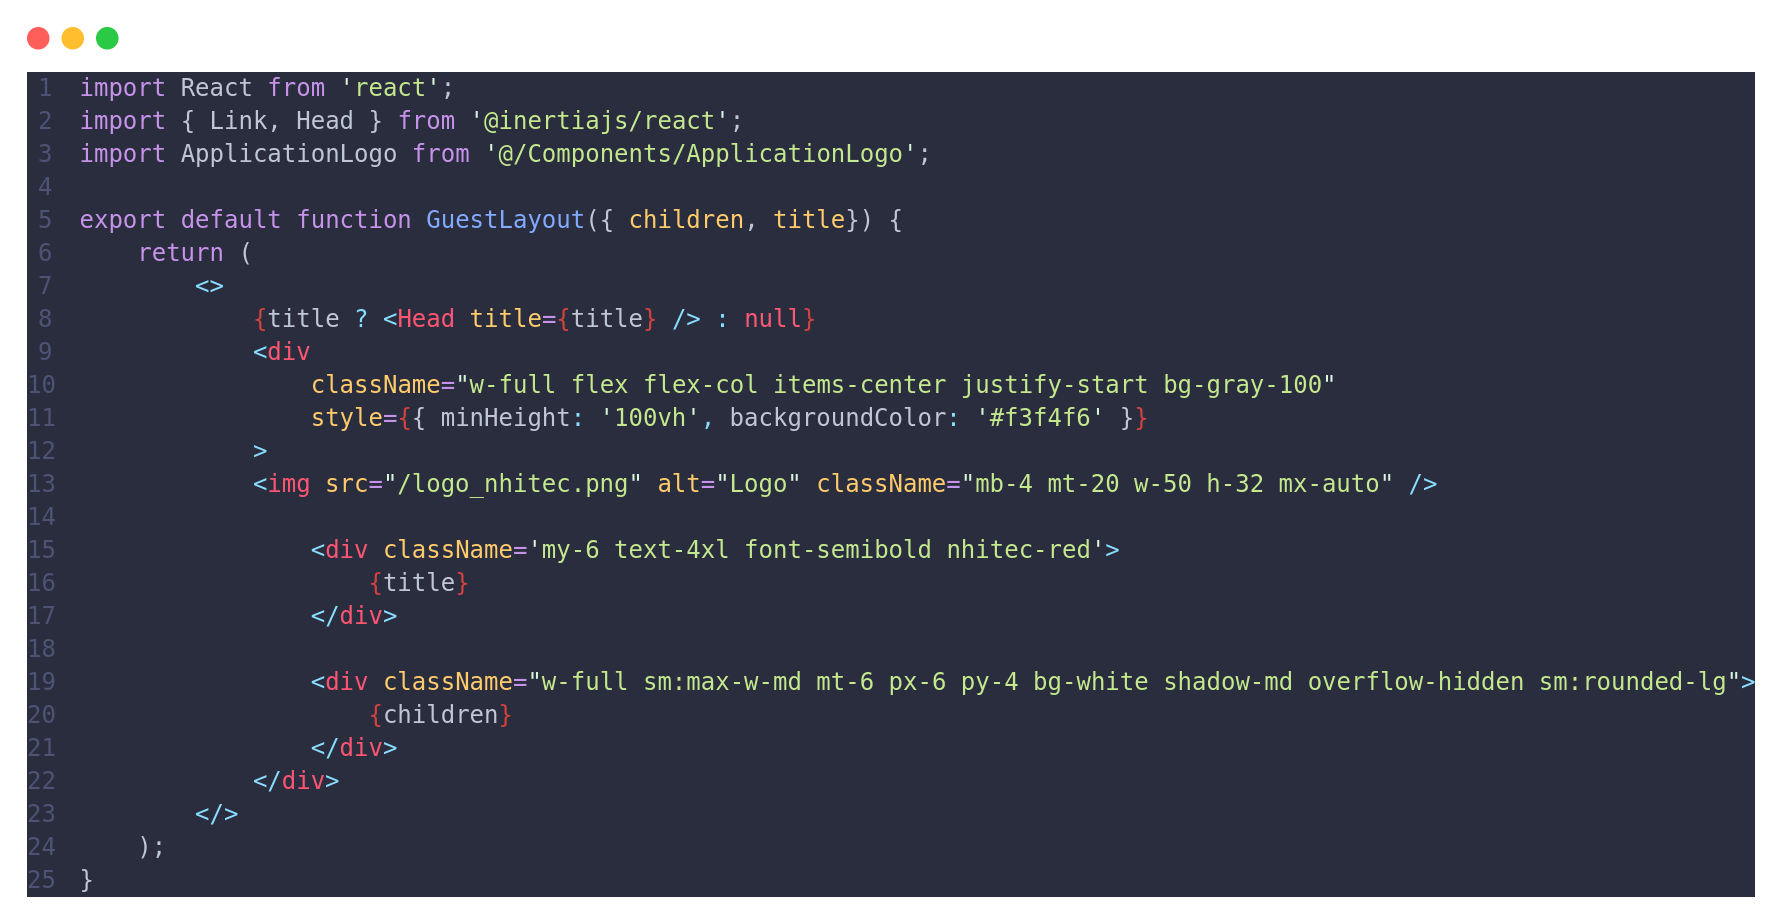
\includegraphics[width=0.8\linewidth]{figures-C1/guestlayout.png}}
    \caption{\texttt{GuestLayout.jsx}}
    \label{fig:guestlayout}
\end{figure}

\newpage

\subsubsubsection[Login]{Login}

\begin{wrapfigure}[7]{r}{0.4\textwidth}
    \vspace{-2.5cm}
    \colorbox{black}{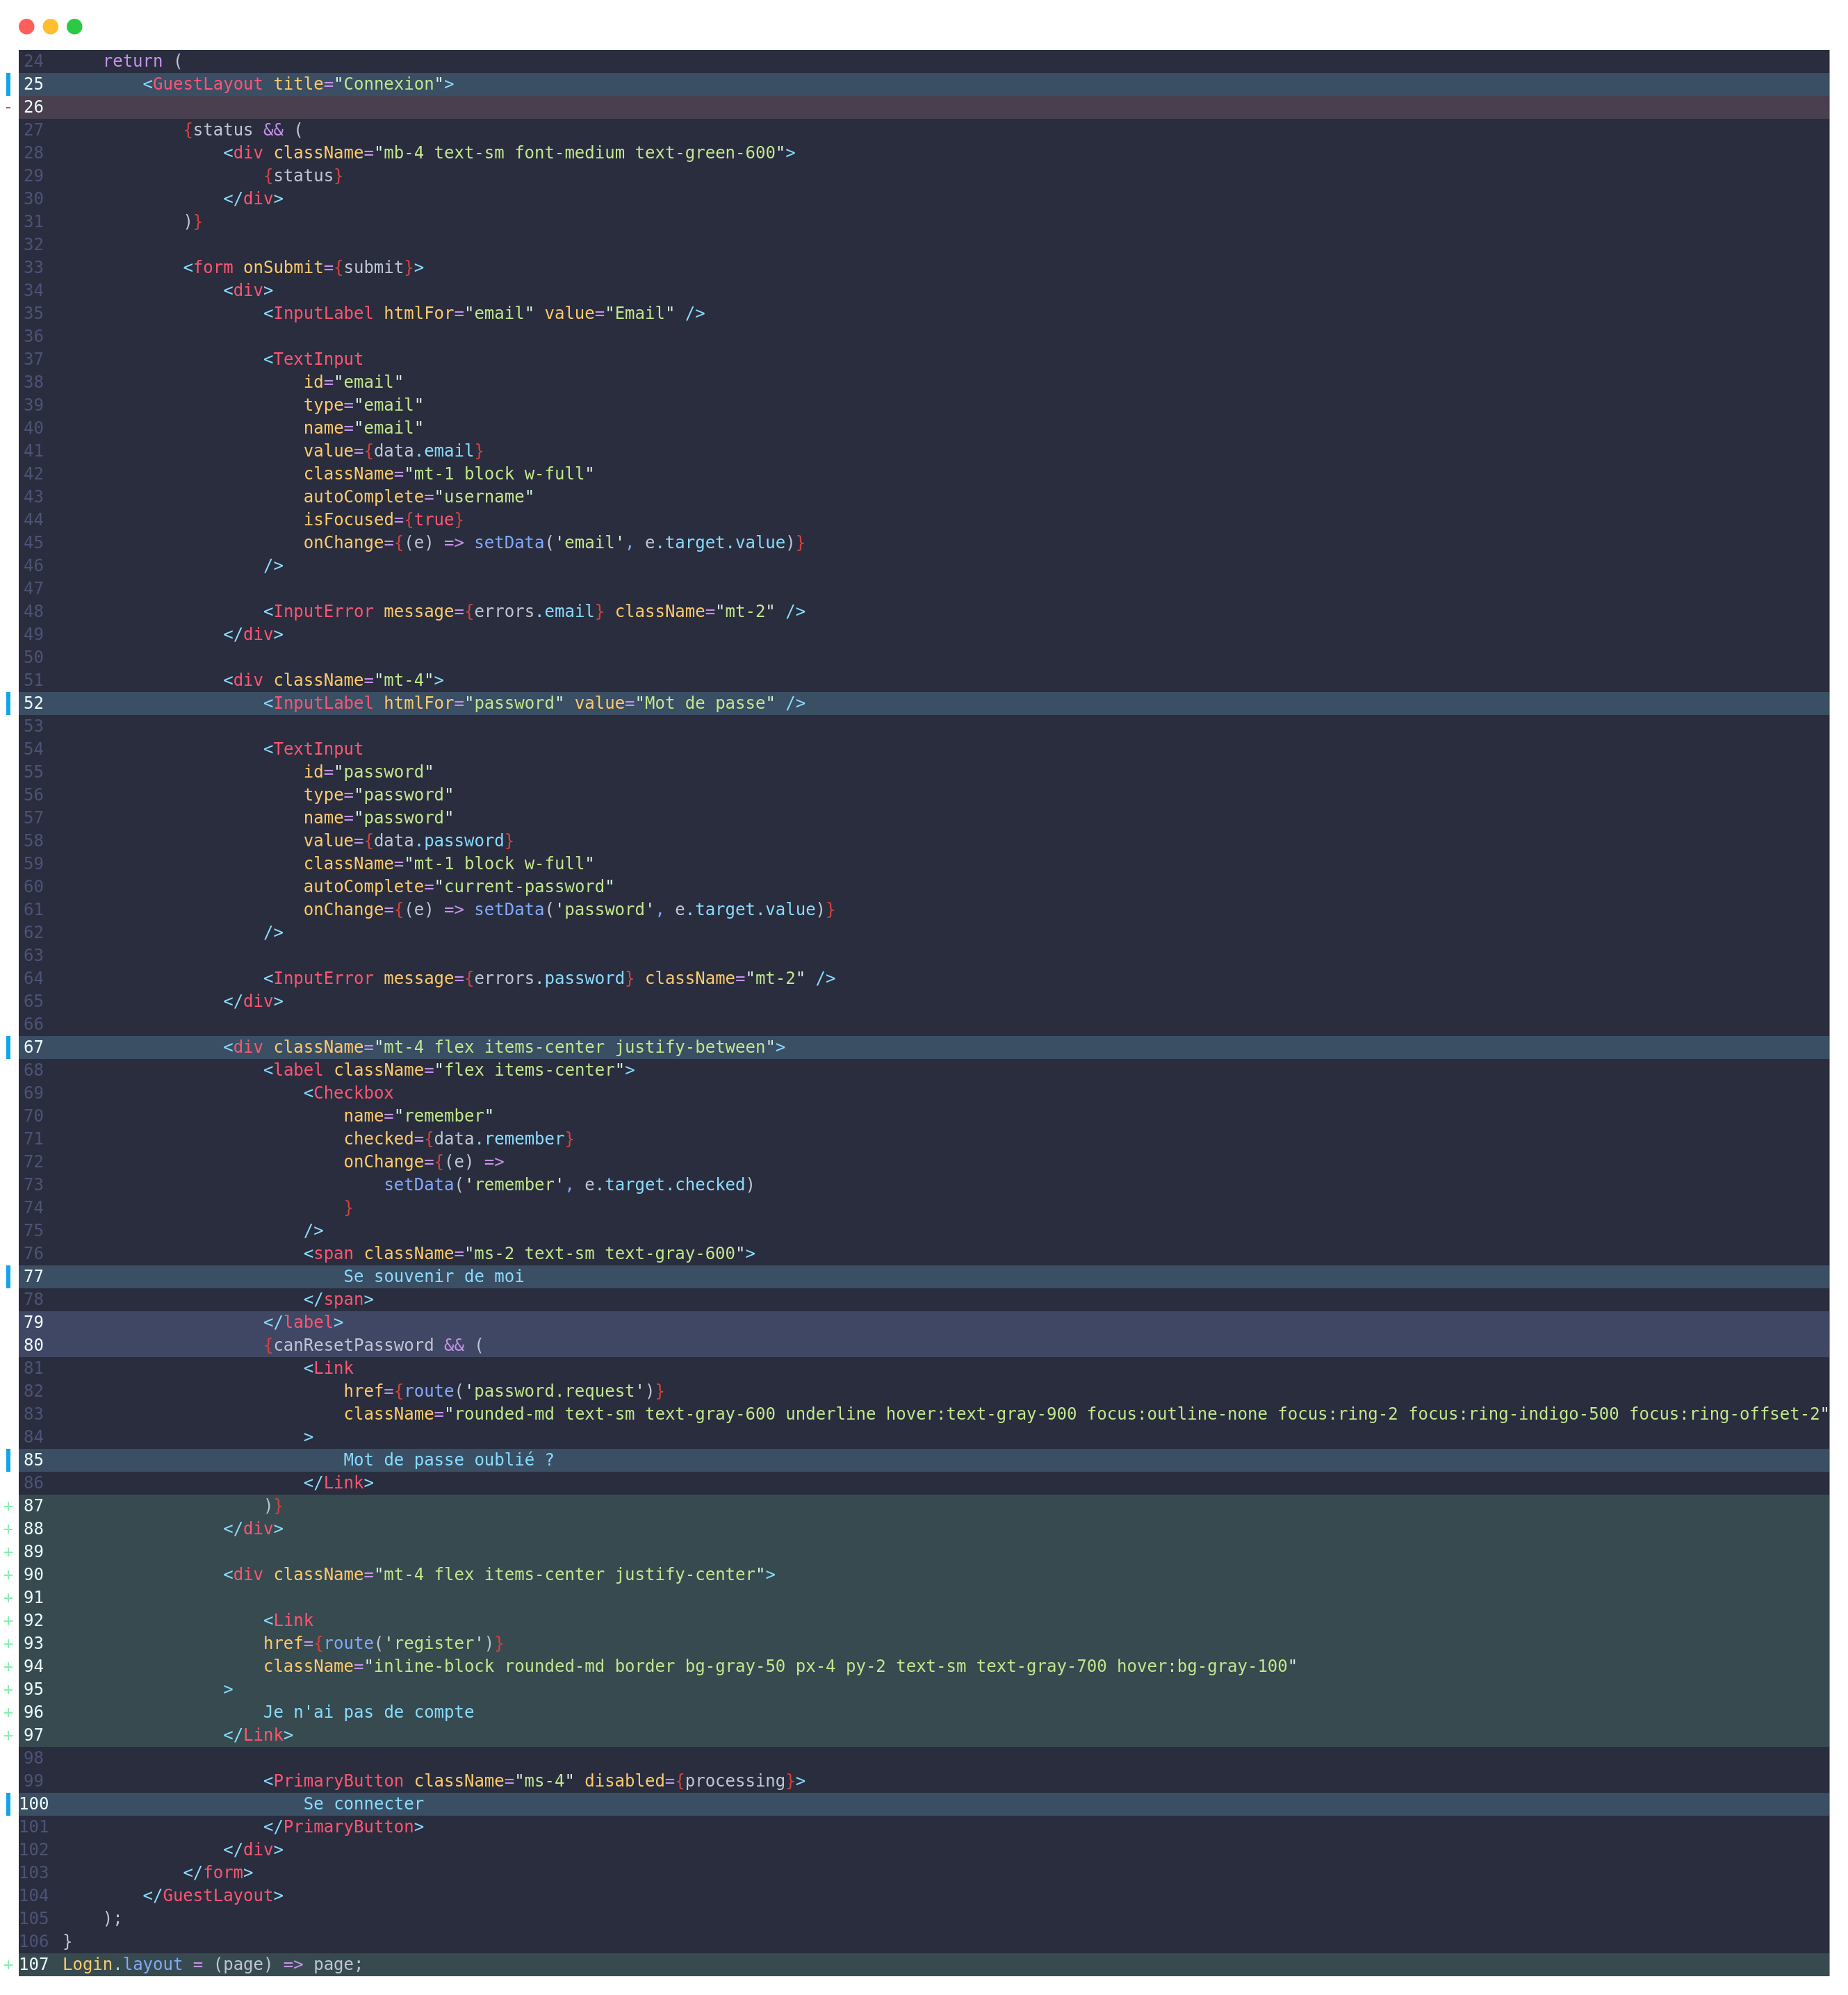
\includegraphics[width=0.4\textwidth]{figures-C1/login.png}}
    \caption{\texttt{Login.jsx}}
\end{wrapfigure}

Nous avons mentionné des pages toutes faites à la section \ref{sec:auth_pages}. Nous allons les modifier en commençant par \texttt{Login.jsx} se trouvant dans le dossier \texttt{resources/js/Pages/Auth}. Apportez-y les modifications suivantes \footnote{Attention à bien supprimer les deux lignes entre 79 et 80 (surlignées en gris sur la figure} :

Nous avons traduit les textes en français, ajouté un bouton "Je n'ai pas de compte" et désactivé le layout principal \texttt{AppLayout.jsx} en fin de fichier \footnote{Oui, souvenez-vous on vient de créer un layout spécial pour les pages de connexion. C'est ce dernier qu'on veut afficher et non pas l'autre qu'on a crée au début de la formation.}.

\subsubsubsection{Register \& ForgotPassword}

Modifiez le fichier comme les figures \ref{fig:register} \& \ref{fig:forgotpassword}

Il n'y a rien à dire de plus là-dessus c'est comme pour \texttt{Login}

\begin{figure}[h]
    \centering
    \begin{minipage}[t]{0.45\textwidth}
        \colorbox{black}{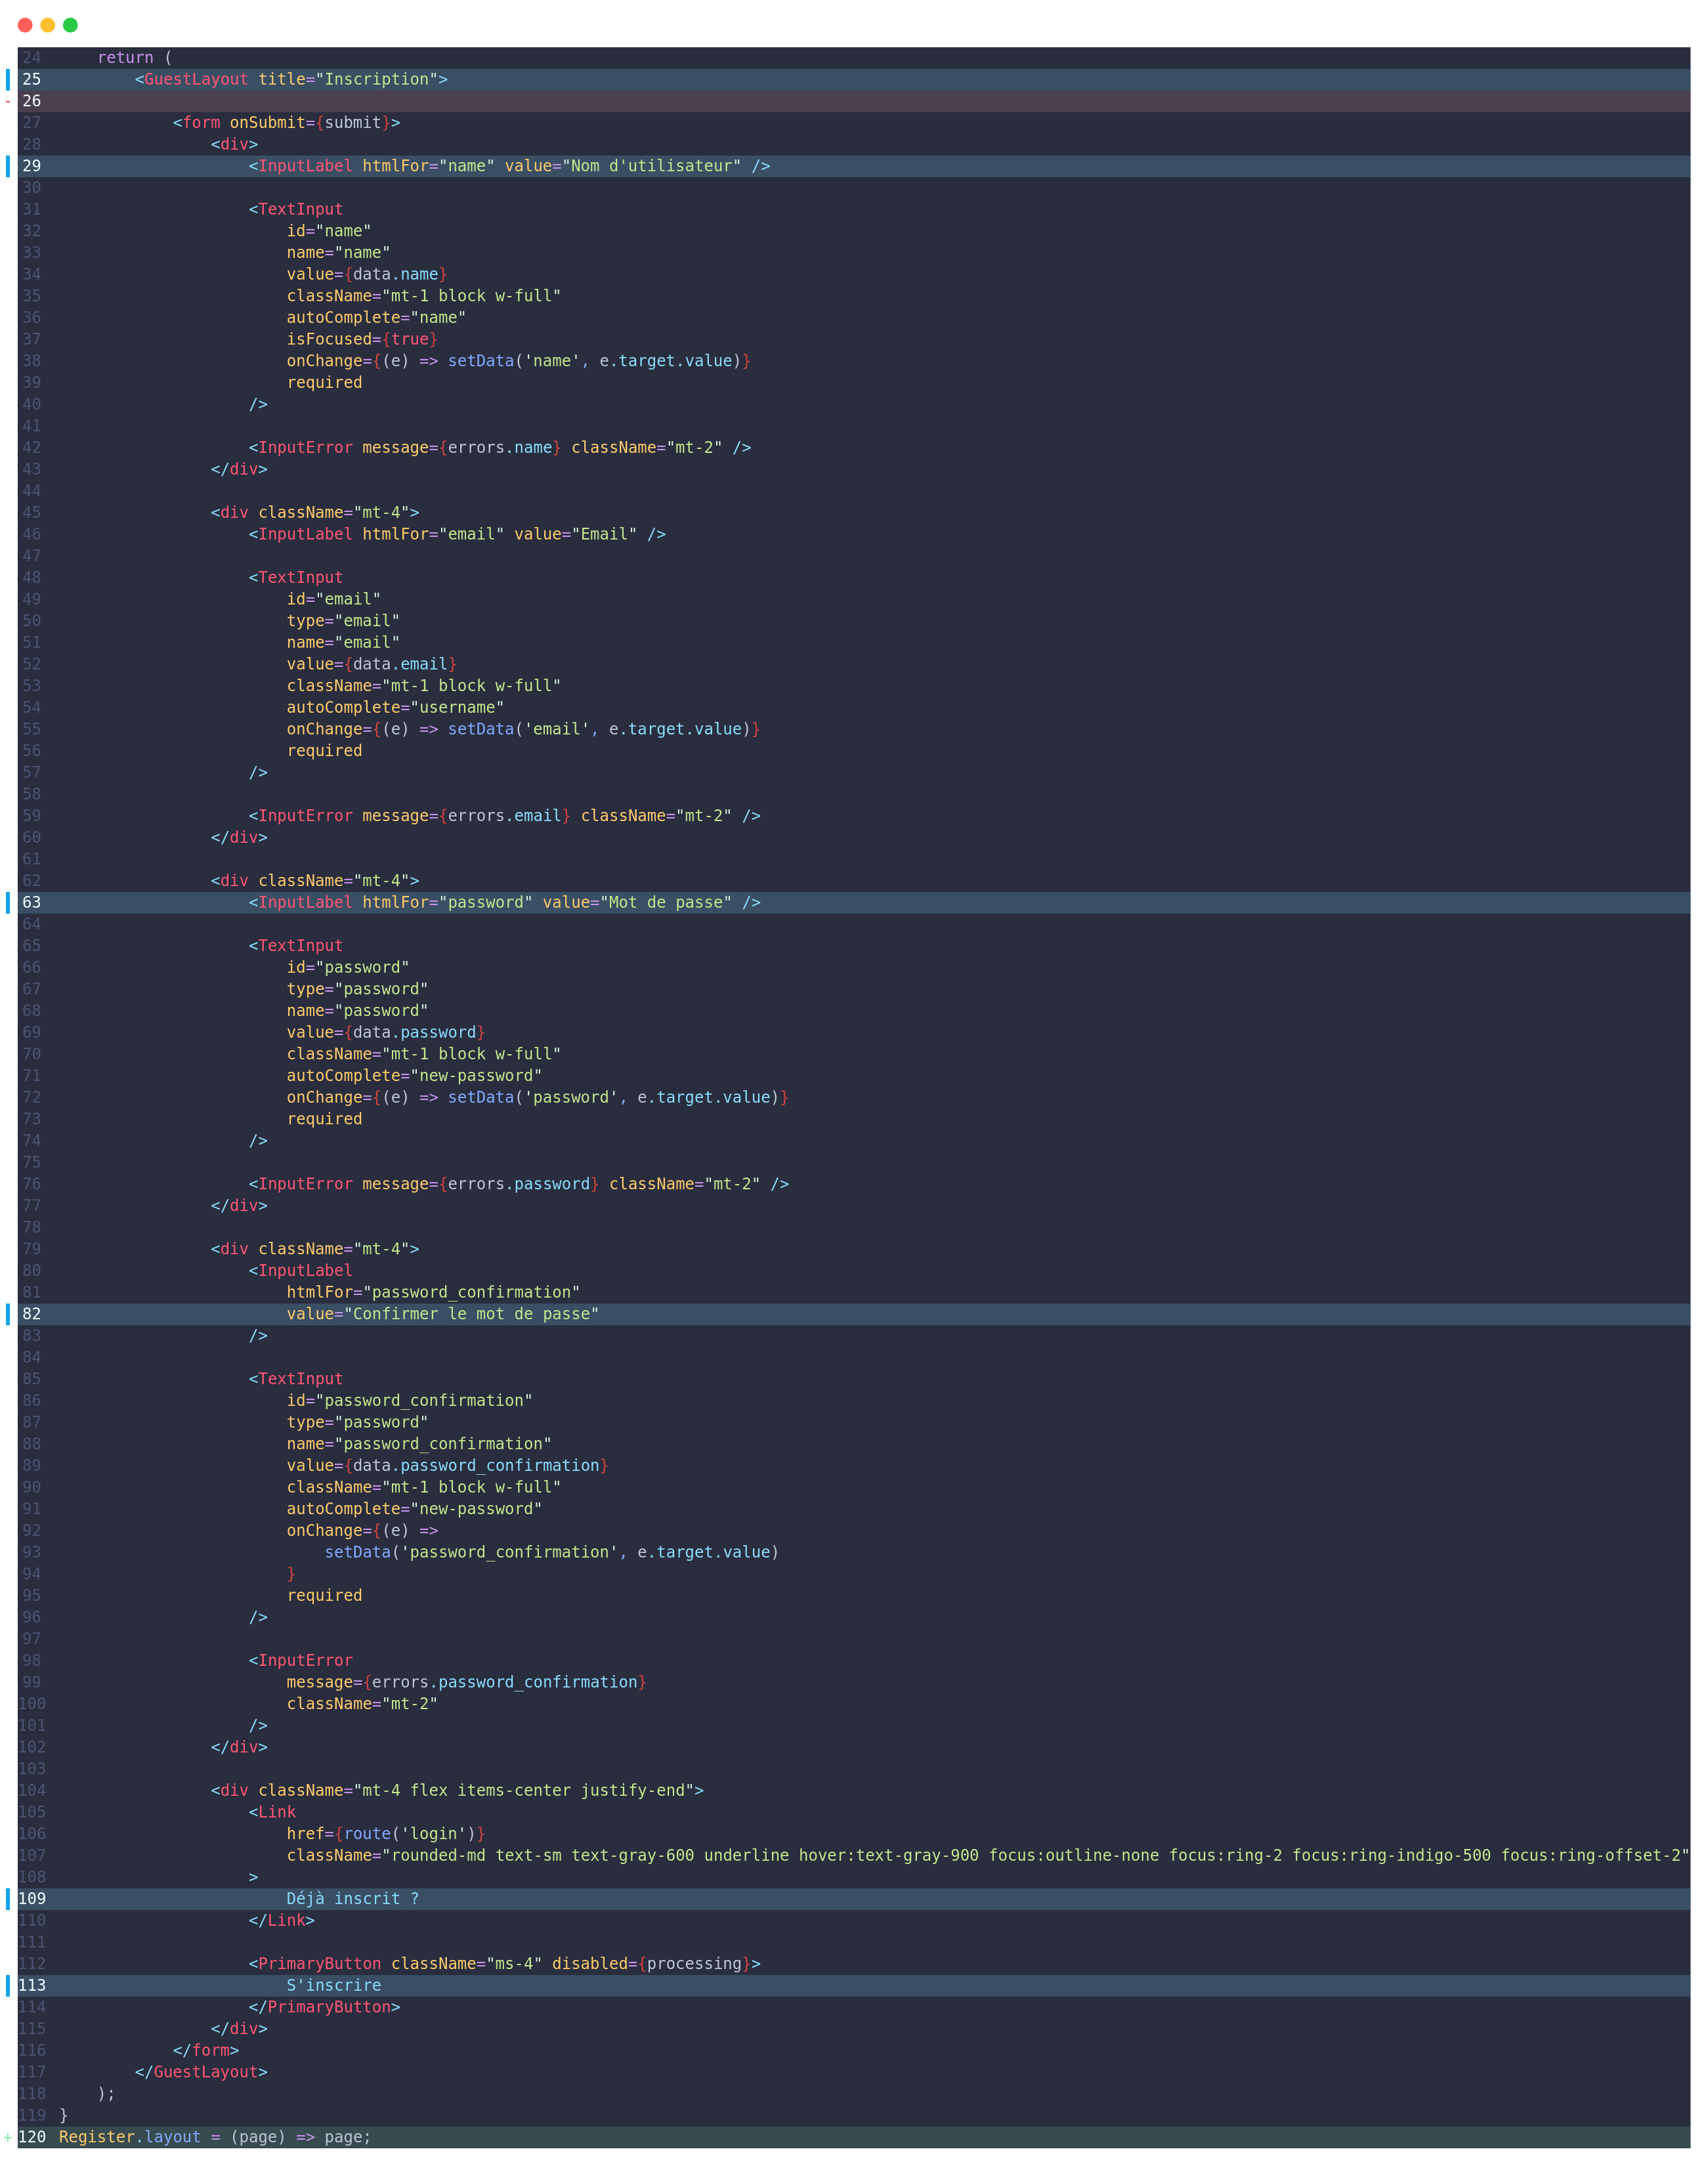
\includegraphics[width=\textwidth]{figures-C1/register.png}}
        \caption{\texttt{Register.jsx}}
        \label{fig:register}
    \end{minipage}
    \hfill
    \begin{minipage}[t]{0.45\textwidth}
        \colorbox{black}{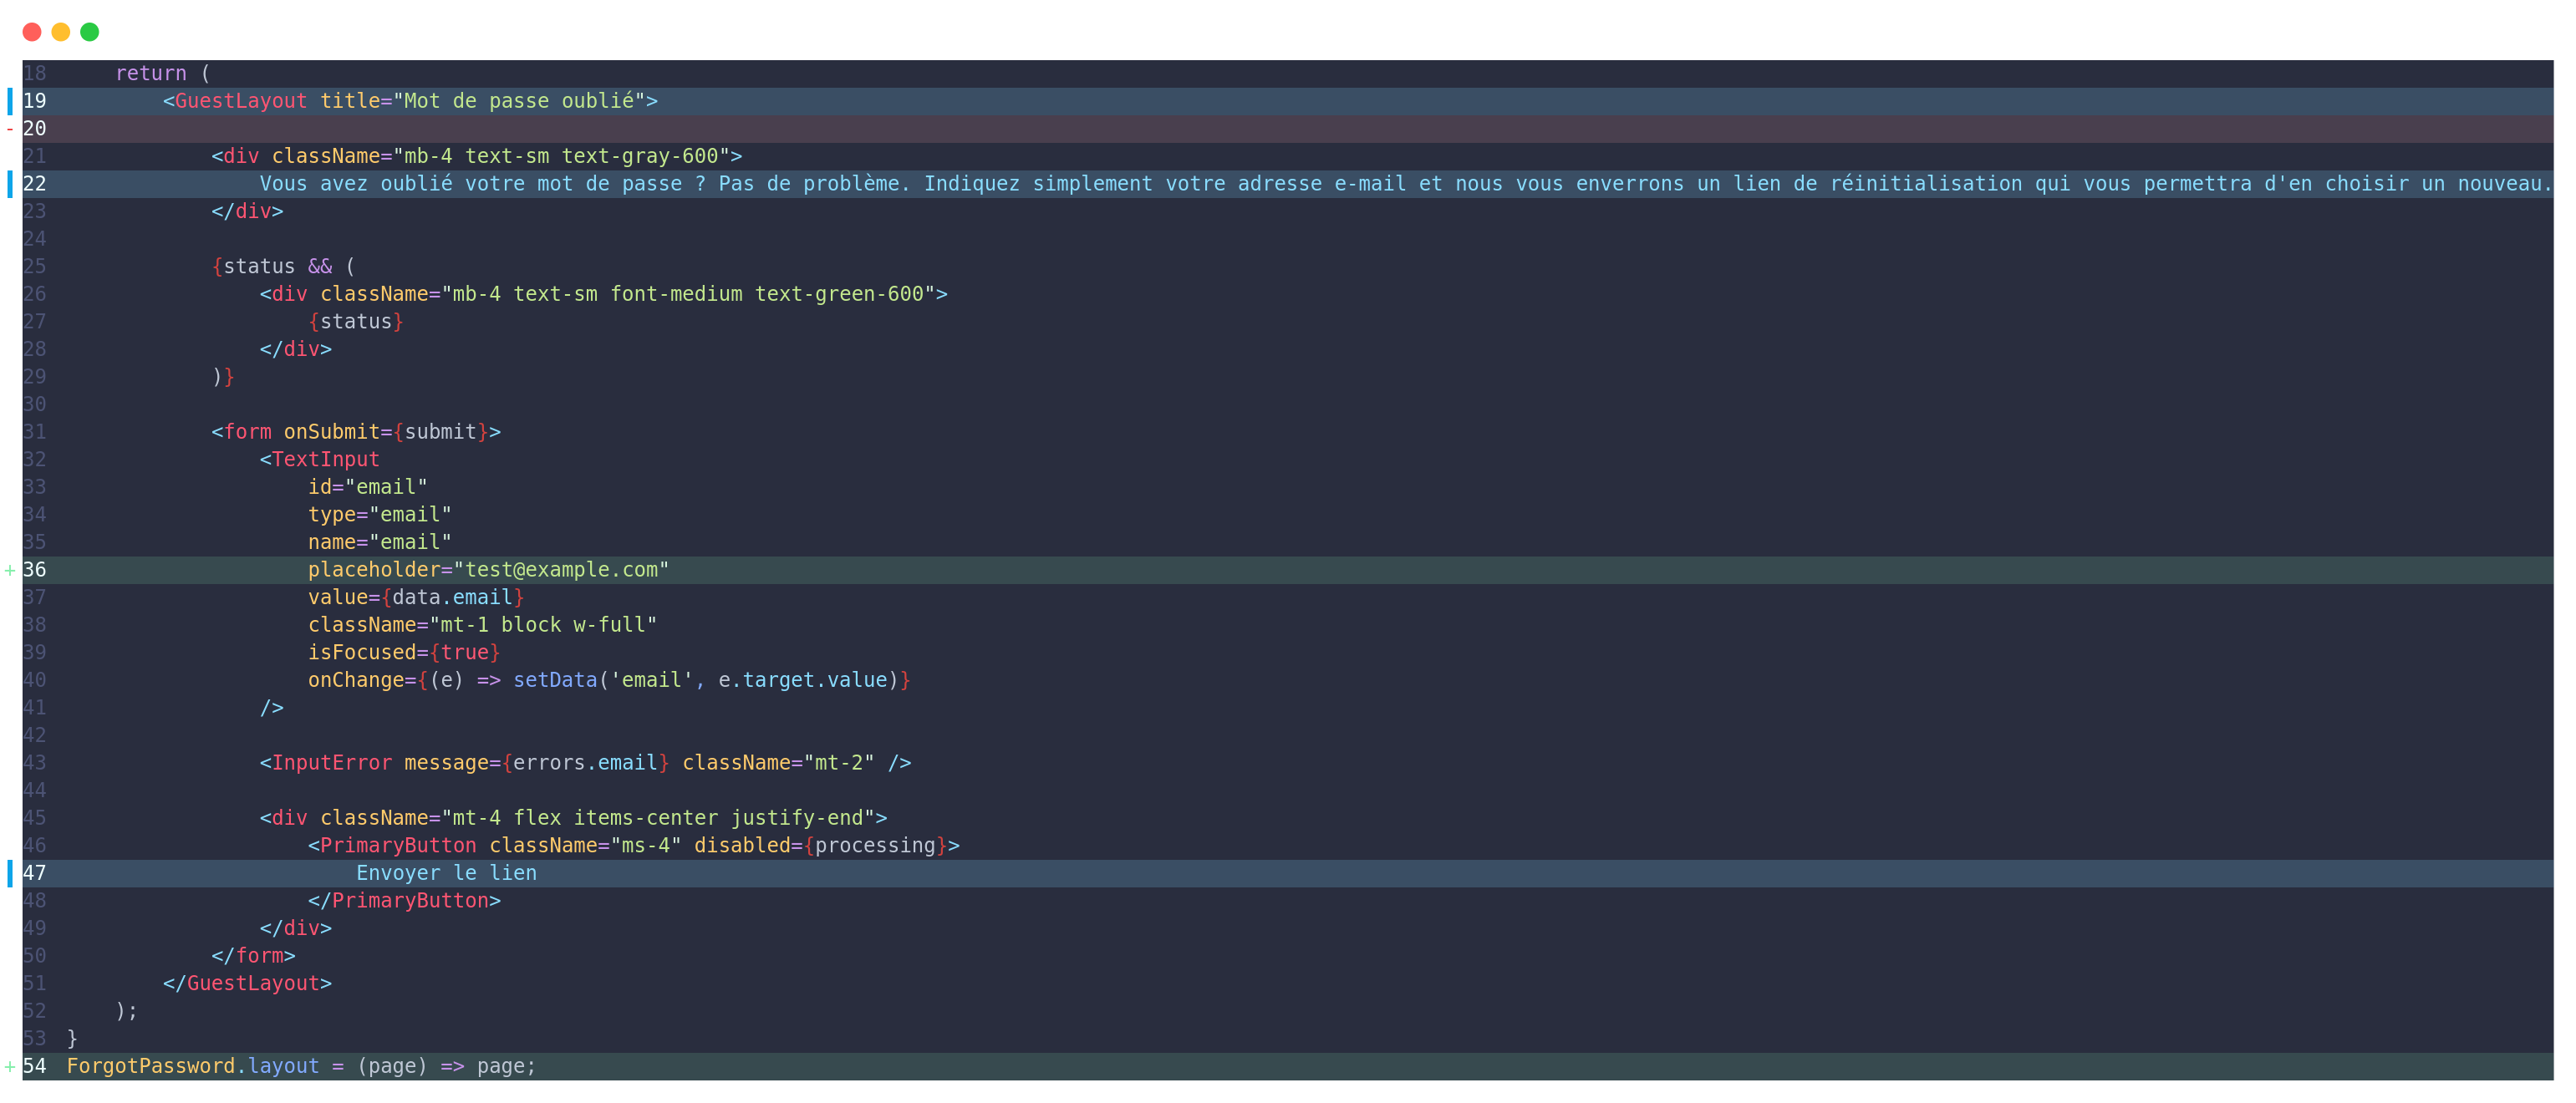
\includegraphics[width=\textwidth]{figures-C1/forgotpassword.png}}
        \caption{\texttt{ForgotPassword.jsx}}
        \label{fig:forgotpassword}
    \end{minipage}
    
\end{figure}

\newpage

\subsubsubsection{Déconnexion}

\begin{wrapfigure}[7]{r}{0.5\textwidth}
    \vspace{-1.5cm}
    \colorbox{black}{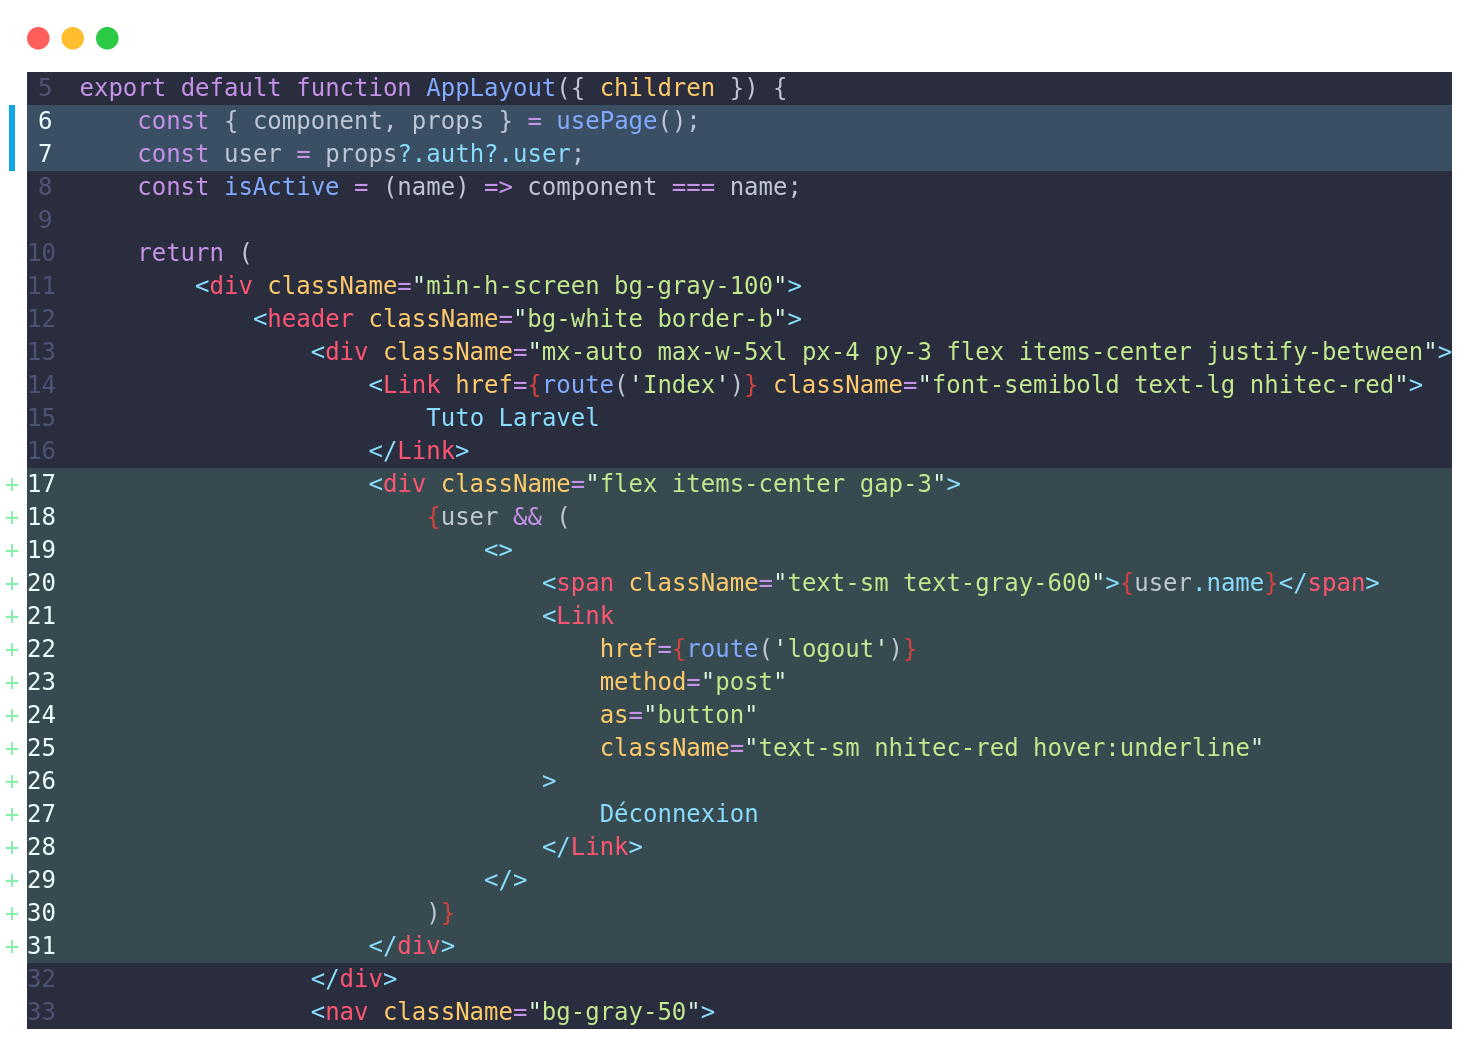
\includegraphics[width=0.5\textwidth]{figures-C1/middleware_applayout.png}}
    \caption{\texttt{AppLayout.jsx}}
\end{wrapfigure}

Maintenant qu'il est possible de se connecter, il faut aussi savoir se déconnecter.

Dans \texttt{resources/js/Layouts/AppLayout.jsx}, ajoutez ceci :

On a ajouté : 
\begin{itemize}
    \item le champ \texttt{user.name} qui va chercher le nom d'utilisateur dans la base de données et l'afficher sur la page \footnote{Comme à la section \ref{sec:utilisation}.}.
    \item un bouton de déconnexion qui redirige vers \texttt{/logout} qui déconnecte l'utilisateur.
\end{itemize}

\subsubsection[Middlewares][laravel.com/docs/12.x/middleware]{Middlewares}\label{sec:middleware}

La formation arrive tout doucement à sa fin. Il nous reste une dernière petite notion à voir, celle du middleware, ou intergiciel en français \footnote{On essaie d'éviter un maximum les anglicismes mais pour des raisons évidentes, nous allons nous tenir à middleware. La France préconise le terme logiciel médiateur mais ce n'est pas beaucoup mieux.}, servant à vérifier si le cookie de session envoyé par l'utilisateur est bien correct \footnote{C'est un peu comme un videur à l'entrée d'une boîte de nuit.}. Si oui, l'utilisateur est connecté.

\begin{wrapfigure}[10]{r}{0.5\textwidth}
    \colorbox{black}{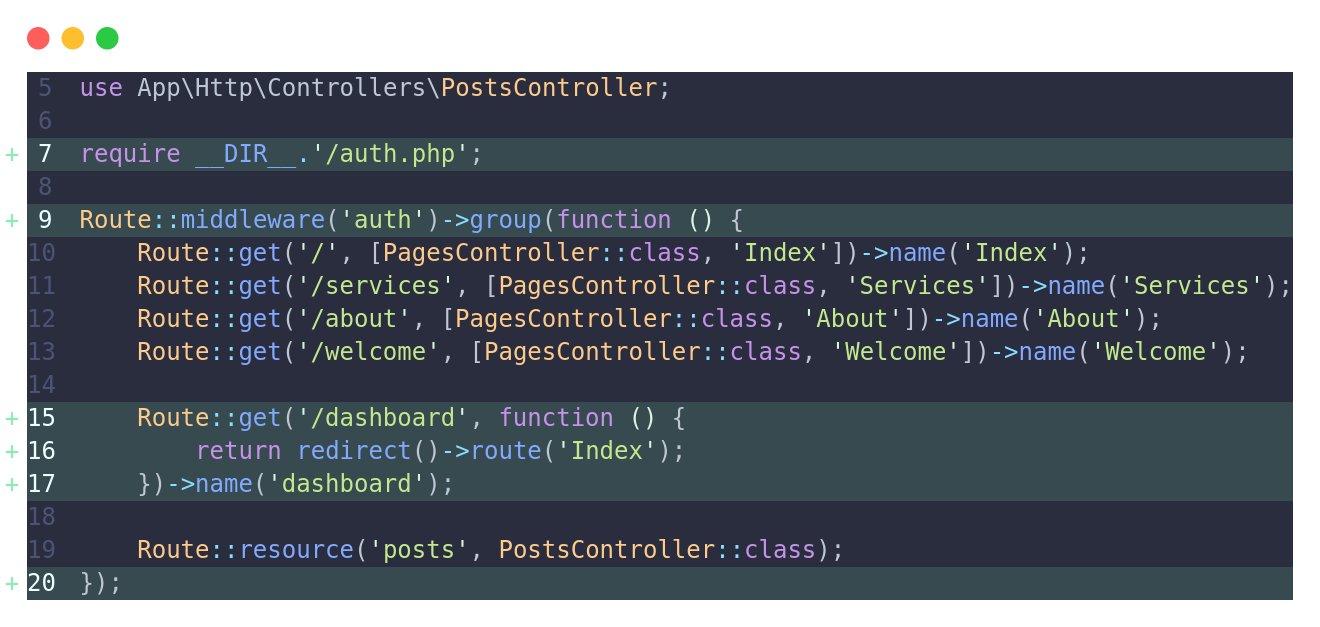
\includegraphics[width=0.5\textwidth]{figures-C1/middleware_web.png}}
    \caption{\texttt{web.php}}
\end{wrapfigure}

Bien ajoutons ce fameux middleware à nos routes pour les protéger. Ajoutez ces lignes dans \texttt{routes/web.php}. Ici, on utilise les routes de \texttt{auth.php} et on ajoute une redirection  vers notre page \texttt{Index} après la connexion \footnote{Par défaut, \laravel redirige vers \texttt{/dashboard} après la connexion. On fait donc une redirection \newline  \texttt{/dashboard -> / }, qui est l'URL de notre page d'accueil.}.

Une fois cela fait, les pages que nous avons créées doivent désormais être protégées par le middleware et vous rediriger vers la page de connexion.

Voilà qui conclut notre formation sur \laravel en utilisant \inertia{} et \react.

\newpage

